% This file was created by matlab2tikz.
%
\documentclass[tikz]{standalone}
\usepackage[T1]{fontenc}
\usepackage[utf8]{inputenc}
\usepackage{pgfplots}
\usepackage{grffile}
\pgfplotsset{compat=newest}
\usetikzlibrary{plotmarks}
\usetikzlibrary{arrows.meta}
\usepgfplotslibrary{patchplots}
\usepackage{amsmath}

\newlength\figureHeight \setlength{\figureHeight}{6cm}
\newlength\figureWidth \setlength{\figureWidth}{10cm}
\begin{document}
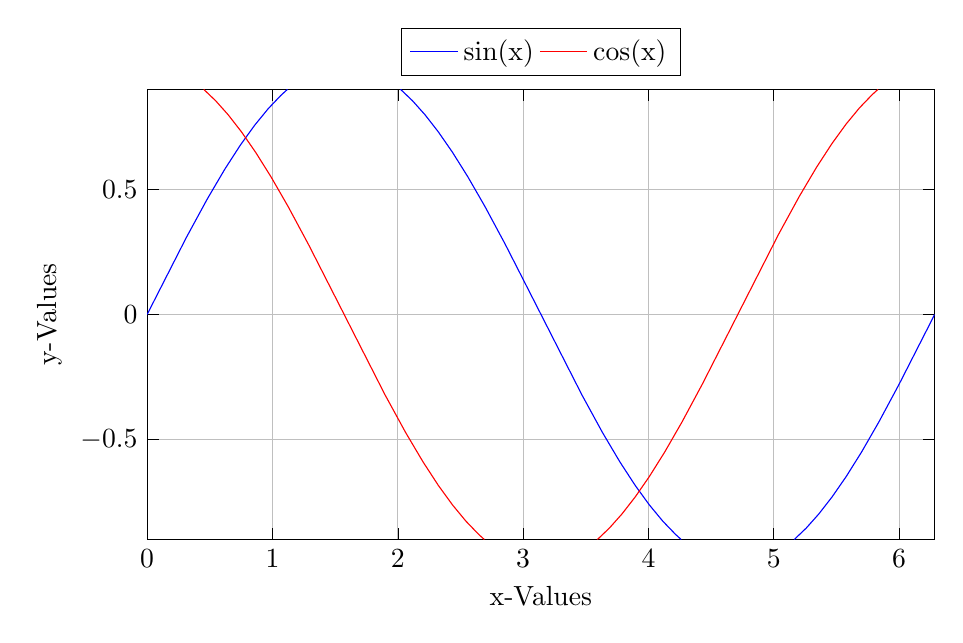
\begin{tikzpicture}

\begin{axis}[%
width=\figureWidth,
height=0.953\figureHeight,
at={(0\figureWidth,0\figureHeight)},
scale only axis,
unbounded coords=jump,
separate axis lines,
every outer x axis line/.append style={black},
every x tick label/.append style={font=\color{black}},
every x tick/.append style={black},
xmin=   0,
xmax=6.28319,
xlabel={${\text{x-Values}}$},
every outer y axis line/.append style={black},
every y tick label/.append style={font=\color{black}},
every y tick/.append style={black},
ymin=-0.9,
ymax= 0.9,
ylabel={${\text{y-Values}}$},
axis background/.style={fill=white},
title style={font=\bfseries},
title={${\text{tikz test}}$},
xmajorgrids,
ymajorgrids,
legend style={at={(0.5,1.03)}, anchor=south, legend columns=2, legend cell align=left, align=left, draw=black}
]
\addplot [color=blue]
  table[row sep=crcr]{%
   0	   0\\
0.313094	0.308004\\
0.480291	0.462038\\
0.619905	0.580958\\
0.744188	0.677375\\
0.858166	0.756645\\
0.964667	0.821859\\
1.06545	0.875007\\
1.1198	0.900013\\
 nan	 nan\\
2.02176	0.900027\\
2.11764	0.854168\\
2.2178	0.797895\\
2.32348	0.729855\\
2.43639	0.648186\\
2.5591	0.550104\\
2.69608	0.430922\\
2.85699	0.280773\\
3.07703	0.0645155\\
3.46911	-0.32169\\
3.63329	-0.472121\\
3.77139	-0.588984\\
3.89473	-0.683934\\
4.00808	-0.762062\\
4.11415	-0.826326\\
4.21455	-0.878617\\
4.26142	-0.900027\\
 nan	 nan\\
5.16338	-0.900013\\
5.25927	-0.854152\\
5.35942	-0.797876\\
5.46517	-0.729791\\
5.57808	-0.648115\\
5.70079	-0.550025\\
5.83777	-0.430836\\
5.99874	-0.280623\\
6.21891	-0.0642334\\
6.28319	  -0\\
};
\addlegendentry{sin(x)}

\addplot [color=red]
  table[row sep=crcr]{%
0.451012	0.900007\\
0.546894	0.854144\\
0.647049	0.797866\\
0.752796	0.72978\\
0.865706	0.648103\\
0.988418	0.550012\\
1.12539	0.430822\\
1.28637	0.280607\\
1.50653	0.0642177\\
1.89817	-0.321557\\
2.06241	-0.472052\\
2.20058	-0.588972\\
2.32392	-0.683923\\
2.43727	-0.762052\\
2.54333	-0.826317\\
2.64374	-0.87861\\
2.69061	-0.90002\\
 nan	 nan\\
3.59257	-0.90002\\
3.68846	-0.85416\\
3.78861	-0.797885\\
3.89429	-0.729845\\
4.0072	-0.648174\\
4.12992	-0.550091\\
4.26689	-0.430907\\
4.4278	-0.280758\\
4.64791	-0.0644372\\
5.03986	0.321646\\
5.20404	0.47208\\
5.34214	0.588946\\
5.46548	0.6839\\
5.57883	0.762031\\
5.68489	0.826299\\
5.7853	0.878595\\
5.83217	0.900007\\
};
\addlegendentry{cos(x)}

\end{axis}
\end{tikzpicture}%
\end{document}